\documentclass[a4paper,12pt]{article}

%%% Размер шрифта
\usepackage[14pt]{extsizes}

%%% Поля
\usepackage[
	left=2cm,
	right=2cm,
	top=2cm,
	bottom=3cm,
	bindingoffset=0cm
]{geometry}

%%% Работа с русским языком
\usepackage{cmap}						% поиск в PDF
\usepackage{mathtext}					% русские буквы в формулах
\usepackage[T2A]{fontenc}				% кодировка
\usepackage[utf8]{inputenc}				% кодировка исходного текста
\usepackage[english,russian]{babel}		% локализация и переносы
\usepackage{indentfirst}
\frenchspacing

%%% Дополнительная работа с математикой
\usepackage{amsmath,amsfonts,amssymb,amsthm,mathtools}  % AMS

%%% Текст в колонки
\usepackage{multicol}

%%% Списки
\usepackage{enumitem}
\setlist{nosep, leftmargin=*}
\renewcommand{\labelenumi}{\arabic*)}

%%% Системы уравнений
\usepackage{cases}

%%% Таблицы
\usepackage{array}

%%% Рисунки
\usepackage{graphicx}
\usepackage{float}

%%% Точка в подписях к рисункам
\usepackage[labelsep=period]{caption}

%%% Список литературы
\bibliographystyle{bibliography_style/gost-numeric.bbx}
\usepackage[
	natbib = true,
	style = gost-numeric,
	sorting = none,
	backend = biber,
	language = autobib,
	autolang = other
]{biblatex}
\addbibresource{references.bib}

%%% Исправление символа номера при использовании gost-numeric.bbx
\usepackage{textcomp}
\DefineBibliographyStrings{russian}{number={\textnumero}}

%%% Гиперссылки
\usepackage[pdftex,unicode]{hyperref}

%%% Перенос знаков в формулах (по Львовскому)
\newcommand*{\hm}[1]{#1\nobreak\discretionary{}{\hbox{$\mathsurround=0pt #1$}}{}}


%%% Свои команды

\newcommand*{\No}{\textnumero}

\newcommand{\vect}[1]{\boldsymbol{#1}}
\newcommand{\vx}{{\vect{x}}}
\newcommand{\vn}{{\vect{n}}}

\newcommand{\half}{\cfrac{1}{2}}

\newcommand{\partt}[1]{\cfrac{\partial #1}{\partial t}}
\newcommand{\partx}[1]{\cfrac{\partial #1}{\partial x}}
\newcommand{\partxx}[1]{\cfrac{\partial^2 #1}{\partial x^2}}
\newcommand{\partvn}[1]{\cfrac{\partial #1}{\partial \vn}}

\newcommand{\partflt}[1]{\partial #1 / \partial t}
\newcommand{\partflx}[1]{\partial #1 / \partial x}
\newcommand{\partflxx}[1]{\partial^2 #1 / \partial x^2}
\newcommand{\partflvn}[1]{\partial #1 / \partial \vn}

\newcommand{\gradsq}[1]{(\nabla #1, \nabla #1)}

\newcommand{\difftau}[1]{\cfrac{{#1}_j^{k + 1} - {#1}_j^k}{\tau}}
\newcommand{\diffhh}[1]{\cfrac{{#1}_{j + 1}^k - 2 {#1}_j^k + {#1}_{j - 1}^k}{h^2}}

\newcommand{\Natural}{{\mathbb{N}}}
\newcommand{\Real}{{\mathbb{R}}}
\newcommand{\bigO}{{\mathcal{O}}}
\newcommand{\clOmega}{{\overline{\Omega}}}

\newcommand{\norm}[1]{\| \, #1 \, \|}
\newcommand{\enorm}{{\| \cdot \|}}

\newcommand{\forcehyphenation}{-\linebreak}

\newcommand{\multeqstart}{
	\begingroup
	\setlength{\abovedisplayshortskip}{\the\abovedisplayskip}
	\setlength{\belowdisplayshortskip}{\the\belowdisplayskip}
}
\newcommand{\multeqnext}{
	\vspace{-7mm}
}
\newcommand{\multeqfinish}{
	\endgroup
}

\newcommand{\absent}[1]{[...#1...]}


%%% Свои операторы
\DeclareMathOperator{\Div}{{div}}
\DeclareMathOperator{\Int}{{Int}}


%%% Оформление теорем

\theoremstyle{plain}
\newtheorem{theorem}{Теорема}
\newtheorem{proposition}{Утверждение}

\theoremstyle{remark}
\newtheorem{remark}{Замечание}


%%% Пояснение к меткам
% eq	-- equation
% cond	-- condition
% char	-- characteristic
% sch	-- scheme
% est	-- estimation
% exp	-- experiment
% fig	-- figure
% tab	-- table
% sec	-- section


%%% Описание препринта
% Комментирование конца строки убирает паразитные пробелы
\newcommand{\PreprintTitle}{%
	Адаптация шага по времени в модели типа <<диффузной границы>>, содержащей уравнение Аллена--Кана%
}
\newcommand{\PreprintTitleFormatted}{%
	Адаптация шага по времени \\ в модели типа <<диффузной границы>>, \\ содержащей уравнение Аллена--Кана%
}
\newcommand{\PreprintTitleEnglish}{
	Time step adaptation in a diffuse interface model including an Allen--Cahn equation%
}
\newcommand{\PreprintAuthors}{%
	А.~С.~Пономарев, Е.~В.~Зипунова, Е.~Б.~Савенков%
}
\newcommand{\PreprintAuthorsEnglish}{%
	A.~S.~Ponomarev, E.~V.~Zipunova, E.~B.~Savenkov%
}


%%%%%%%%%%%%%%%%%%%%%%%%%%%%%%%%%%%%%%%%%%%%%%%%%%%%%%%%%%%%%%%%%%%%%%%%%%%%%%%%

\begin{document}

%%%%%%%%%%%%%%%%%%%%%%%%%%%%%%%%%%%%%%
\begin{titlepage}

\begin{center}
	РОССИЙСКАЯ АКАДЕМИЯ НАУК \\
	ОРДЕНА ЛЕНИНА \\
	ИНСТИТУТ ПРИКЛАДНОЙ МАТЕМАТИКИ \\
	имени М. В. КЕЛДЫША \par

	\vspace*{60mm}
	{
		\Large{\PreprintAuthors} \par
	}
	\vspace*{20mm}
	{
		\large \textbf{\PreprintTitleFormatted} \par
	}
	\vspace*{\fill}
	\Large{Москва, 2025}
	\vspace*{-15mm}
\end{center}

\end{titlepage}
%%%%%%%%%%%%%%%%%%%%%%%%%%%%%%%%%%%%%%%

\setcounter{page}{2}

\thispagestyle{empty}

\noindent \emph{\PreprintAuthors,} \PreprintTitle \\[3mm]
\textbf{Аннотация} \par
{
	\noindent \small
	В работе исследованы три различных подхода к адаптации шага по времени в модели развития канала электрического пробоя типа диффузной границы. Один из подходов предложен авторами настоящей работы, дано его теоретическое обоснование. Для всех трех алгоритмов адаптации проведены численные эксперименты; выявлен наиболее эффективный из них. \\
	Исследованные алгоритмы адаптации универсальны – они могут использоваться и в других моделях типа диффузной границы с уравнением Аллена–Кана. \\[3mm]
	\textbf{Ключевые слова:} модель типа диффузной границы, уравнение Аллена--Кана, адаптация шага по времени \par
	\vspace{5mm}
}
\begin{otherlanguage}{english}
\noindent \emph{\PreprintAuthorsEnglish,} \PreprintTitleEnglish \\[3mm]
\textbf{Abstract} \par
{
	\noindent \small
	\absent{Annotaceaya rabotea na angliyskom} \\[3mm]
	\textbf{Key words and phrases:} diffuse interface model, Allen--Cahn equation, adaptive time-step\-ping method \par
	\vspace{5mm}
}
\end{otherlanguage}

\clearpage

%!TEX root = ../main.tex

\section{Введение}

Электрический пробой~-- это явление резкого возрастания тока в диэлектрике при приложении электрического напряжения выше некоторого критического значения. Механизм разрушения диэлектрика под действием электрического поля сложен и многообразен: оно может иметь различные причины, характер развития, сопутствующие физические процессы \cite{vorobiev_dielectric_physics}.

Среди многообразия математических моделей, созданных для описания развития канала электрического пробоя, выделим предложенную в работе \cite{pitike_dielectric_breakdown} модель типа диффузной границы.

В настоящее время модели типа диффузной границы составляют целый класс подходов для решения задач в различных областях науки и техники. В частности, описанная в работе \cite{pitike_dielectric_breakdown} модель построена как формальное обобщение ранее известных моделей типа диффузной границы, применяемых в теории трещин.

Исследование и дальнейшее развитие упомянутой модели можно найти в работах \cite{zipunova_higher_codimension, zipunova_conservative, zipunova_thermomechanical, ponomarev_stability}. Основные положения метода диффузной границы в применении к моделированию развития канала электрического пробоя перечислены в работе \cite{ponomarev_stability}.

Модели типа диффузной границы используются для описания систем, в которых вещество может находиться в нескольких различных состояниях~-- фазах,~-- причем вещество в одной и той же фазе образует некоторые однородные области. В моделях типа диффузной границы распределение фаз вещества задается гладкой функцией $\phi$~-- фазовым полем,~-- которая в каждой области однородности близка к постоянной. Характерная толщина разделяющего слоя (<<диффузной границы>>) и, соответственно, скорость изменения~$\phi$ при переходе от одной фазы к другой определяется параметрами модели.

В работе \cite{zipunova_higher_codimension} проводится исследование свойства упомянутой модели развития канала электрического пробоя, которое можно назвать коразмерностью <<включений>>. Для задач теории трещин естественным будет двумерное включение (плоская трещина) в трехмерной среде вещества~-- в таком случае говорят, что коразмерность объекта равна 1. Обратим внимание, что, хотя исследуемая модель, как было сказано, получена на основе моделей из теории трещин, для нее характерным будет одномерное включение (канал пробоя), то есть имеющее коразмерность 2. В работе \cite{zipunova_higher_codimension} указано, что это может привести к нетривиальным последствиям, и предложено определенное обобщение исходной модели, которое предположительно делает ее более адекватной.

Суть обобщения состоит в формальном добавлении в уравнения модели двух слагаемых высших порядков с некоторыми коэффициентами. Целью настоящей работы является численная проверка поведения модели при различных значениях коэффициентов. Для этого ищется стационарное распределение фазового поля $\phi$ в нескольких характеристических случаях. Построение разностной схемы для задачи несет определенные сложности, связанные с необходимостью задать граничные условия на множествах коразмерности~2 и~3 в трехмерном пространстве. Предполагается, что точках этих множеств функция фазового поля $\phi$ имеет особенность.

Авторами применена модификация метода конечных объемов. Для части конфигураций обобщенной модели она позволила составить разнотную схему. Создана компьютерная программа, реализующая схему; проделаны расчеты, их результаты приведены в виде графиков. Для остальных конфигураций модели в процессе применения метода возникли фундаментальные проблемы, что позволяет выдвинуть гипотезу о некорректной постановке дифференциальной задачи в этих случаях.

%!TEX root = ../main.tex

\section{Математическая модель}

Приведем краткое описание исследуемой математической модели. По\forcehyphenation дробное описание физического смысла уравнений и параметров модели можно найти в работе \cite{ponomarev_stability}.

Рассматривается ограниченная область пространства $\Omega \subset \Real^3$. Распределение фаз вещества в ней задается гладкой функцией $\phi: \Omega \times [0, +\infty)_t \hm \to [0, 1], \; \phi(\vx, t)$~-- фазовым полем; вещество может находиться в одной из двух фаз: $\phi \approx 1$~-- <<неповрежденное>>, $\phi \approx 0$~-- <<полностью разрушенное>> (то есть относящееся к каналу пробоя),~-- а также в промежуточных состояниях в зоне диффузной границы.

Диэлектрическая проницаемость среды $\epsilon$ задается следующей формулой:
\[
	\epsilon(\vx, t) = \epsilon[\phi] = \cfrac{\epsilon_0(\vx)}{f(\phi(\vx, t)) + \delta}.
\]
Здесь $\epsilon_0(\vx)$~-- диэлектрическая проницаемость неповрежденной среды, $f(\phi) \hm = 4\phi^3 - 3\phi^4$~-- интерполирующая функция, $0 < \delta \ll 1$~-- регуляризующий параметр. Запись $\epsilon[\phi]$ означает функциональную зависимость $\epsilon$ от $\phi$.

Помимо фазового поля $\phi$, состояние системы описывает функция $\Phi: \Omega \hm \times [0, +\infty)_t \to \Real, \; \Phi(\vx, t)$~-- потенциал электрического поля.

Постулируется следующее выражение для свободной энергии системы $\Pi$:
\begin{gather*}
	\Pi = \int \limits_\Omega \pi d \vx, \\
	\pi = -\half \epsilon[\phi] \gradsq{\Phi} + \Gamma \cfrac{1 - f(\phi)}{l^2} + \cfrac{\Gamma}{4} \gradsq{\phi}.
\end{gather*}
Здесь $\Gamma > 0$, $l > 0$~-- числовые параметры модели, константы.

Постулируются два уравнения, определяющие динамику системы:
\begin{equation*}
\begin{cases}
	\cfrac{\delta \Pi}{\delta \Phi} = 0; \\[3mm]
	\cfrac{1}{m} \partt{\phi} = -\cfrac{\delta \Pi}{\delta \phi}.
\end{cases}
\end{equation*}
Здесь константа $m > 0$~-- числовой параметр модели, называемый подвижностью. Говоря нестрого, согласно первому уравнению электрический потенциал $\Phi$ распределяется так, чтобы свободная энергия была минимальной; согласно второму~-- фазовое поле $\phi$ с определенной скоростью стремится к тому, чтобы свободная энергия была минимальной.

Отыскав явно вариационные производные в двух уравнениях выше, получим следующую систему уравнений:
\begin{numcases}{}
	\Div(\epsilon[\phi] \nabla \Phi) = 0;
	\label{eq:Phi} \\
	\cfrac{1}{m} \partt{\phi} = \half \epsilon'(\phi) \gradsq{\Phi} + \cfrac{\Gamma}{l^2} f'(\phi) + \half \Gamma \Delta \phi.
	\label{eq:phi}
\end{numcases}
Здесь $(\cdot)' \equiv (\cdot)_\phi'$. Система состоит из двух уравнений: на $\phi$ и $\Phi$ соответственно; система связная.

Уравнение \eqref{eq:phi} имеет вид
\[
	\cfrac{1}{m} \partt{\phi} = -F'(\phi; |\nabla \Phi|) + \half \Gamma \Delta \phi,
\]
где
\begin{equation}
	F(\phi; |\nabla \Phi|) = -\half \epsilon[\phi] |\nabla \Phi|^2 + \Gamma \cfrac{1 - f(\phi)}{l^2}
	\label{eq:allen_cahn_potential}
\end{equation}
есть определенная нелинейная функция от $\phi$, которая к тому же зависит от~$|\nabla \Phi|$ как от параметра. Таким образом, перед нами нелинейное уравнение типа Аллена--Кана. \absent{Ссылка}

Из вывода модели очевидна следующая запись формулы для плотности свободной энергии:
\begin{equation}
	\pi = F(\phi; |\nabla \Phi|) + \cfrac{\Gamma}{4} \gradsq{\phi}.
	\label{eq:energy_density}
\end{equation}

В классической постановке Аллена--Кана $F$ -- двухъямный потенциал. В рассмотриваемой задаче $F$ меняет поведение в зависимости от значения~$|\nabla \Phi|$, как было показано в работе \cite{ponomarev_stability}. Возможны три случая в зависимости от величины
\[
	\xi = \cfrac{|\nabla \Phi|^2 l^2 \epsilon_0}{2 \Gamma},
\]
а именно:
\begin{itemize}
	\item \makebox[5.3cm][l]{<<слабое напряжение>>,} \makebox[4.0cm][l]{$\xi < \delta^2$:} $F(\phi)$ монотонно убывает;
	\item \makebox[5.3cm][l]{<<среднее напряжение>>,} \makebox[4.0cm][l]{$\delta^2 < \xi < (1 + \delta)^2$:} $F(\phi)$ унимодальна, убывание \par {\raggedleft сменяется возрастанием; \par}
	\item \makebox[5.3cm][l]{<<сильное напряжение>>,} \makebox[4.0cm][l]{$\xi > (1 + \delta)^2$:} $F(\phi)$ монотонно возрастает.
\end{itemize}
Наибольший интерес для практики моделирования представляет случай \linebreak <<сильного напряжения>>, так как именно тогда канал пробоя развивается из сколь угодно малых возмущений неповрежденной среды.

%!TEX root = ../main.tex

\section{Finite difference scheme}
\label{sec:differential_scheme}

In this section we present finite-difference scheme for solution of
the equation~\eqref{eq:one_dim} in the domain~$[0, W]_x \times [0,
+\infty)_t$
subjected to initial conditions~\eqref{eq:one_dim_initial} and boundary conditions~\eqref{eq:one_dim_marginal}.

Consider regular mesh with time step~$\tau$ and
spatial mesh step size~$h$. Let~$W = Nh$ with $N$ being number of
nodes. Nodes of spatiotemporal grid are given by~$(jh, k \tau)$,
$j = \overline{0, N}$, $k \in \Natural_0$. Define by~$\phi_j^k$
a value of mesh function~$\phi$ at the node~$(jh, k \tau)$.
Then the finite-difference approximations read
\begin{equation}
  \cfrac{1}{m} \difftau{\phi} = \half K_\phi^2 \epsilon'(\phi_j^k) + \cfrac{\Gamma}{l^2} f'(\phi_j^k) + \cfrac{\Gamma}{2} \diffhh{\phi} \tpoint
  \label{eq:subtractive}
\end{equation}
or, in the explicit form,
\begin{gather}
  \begin{aligned}
    \phi_j^{k + 1} = \phi_j^k + m \tau \left( \half K_\Phi^2 \epsilon'(\phi_j^k) + \cfrac{\Gamma}{l^2} f'(\phi_j^k) + \cfrac{\Gamma}{2} \diffhh{\phi} \right), \\ j = \overline{1, N - 1}, \quad k \in \Natural_0 \tsemicolon
  \end{aligned}
  \label{sch:transition} \\
  \phi_j^0 = \phi_0(jh); \quad \phi_0^k = \phi_l(k \tau); \quad \phi_N^k = \phi_r(k \tau) \tpoint
  \label{sch:borders}
\end{gather}

It is easy to see the scheme is of the first order of approximation in
time and second order approximation in spatial terms.

To study properties of the scheme~\eqref{sch:transition}, \eqref{sch:borders}
the linear theory can be used (see, e.g.,
\cite[Chapter~10]{bahvalov_computational_methods}
or~\cite[Chapter~IX]{kalitkin_computational_methods}).
The central result of the theory states, in a somewhat simplified
form, that if a finite-difference scheme is stable and approximate
continuous problem, then solution of the finite-dimensional problem
converges to the solution of the continuous one with the order
not lower then order of approximation.

To apply this result for the nonlinear setting~\eqref{sch:transition}, \eqref{sch:borders} at
hand we proceed in the following way:
(i) linearize equation~\eqref{eq:subtractive}
for fixed~$\phi$, and then (ii) apply spectral stability argument~\cite{bahvalov_computational_methods} to the
derived linearized equation. As stability criteria will be
satisfied for the linearized equation, it should be expected for the
complete, nonlinear, problem. In this case convergence of the
approximate solution should be expected as well~--- since
the finite-difference problem is stable and approximate the continuous
one.
The results of such non-rigorous analysis will be further confirmed by
numerical computations in the fully nonlinear setting.


\subsection{Stability estimate}

In this section we derive  stability condition for
finite-difference scheme~\eqref{sch:transition}, \eqref{sch:borders}
using the so called principal of the ``frozen coefficients''
(see, e.g.,~\cite{bahvalov_computational_methods}).
Let~$\phi_j^k$ and~$\phi_j^k + \delta_j^k$ be solutions of the
finite-difference equation~\eqref{eq:subtractive}.
Substitute~$\phi_j^k + \delta_j^k$ into~\eqref{eq:subtractive} to obtain:
\begin{multline*}
  \cfrac{1}{m} \cfrac{(\phi_j^{k + 1} + \delta_j^{k + 1}) - (\phi_j^k + \delta_j^k)}{\tau} = \half K_\Phi^2 [\epsilon'(\phi_j^k) + \epsilon''(\phi_j^k) \delta_j^k + o(\delta_j^k)] + \\ + \cfrac{\Gamma}{l^2} [f'(\phi_j^k) + f''(\phi_j^k) \delta_j^k + o(\delta_j^k)] + \cfrac{\Gamma}{2} \cfrac{(\phi_{j + 1}^k + \delta_{j + 1}^k) - 2 (\phi_j^k + \delta_j^k) + (\phi_{j - 1}^k + \delta_{j - 1}^k)}{h^2} \tpoint
\end{multline*}
Linearizing this equation around~ $\phi_j^k = P$, assuming that
perturbations~$\delta_j^k$ are small, and taking into account
that~$\phi_j^k$ is a solution of the finite-difference problem, one
arrives to:
\begin{equation}
  \delta_j^{k + 1} = \delta_j^k + m \tau \left( \half K_\Phi^2 \epsilon''(P) \delta_j^k + \cfrac{\Gamma}{l^2} f''(P) \delta_j^k + \cfrac{\Gamma}{2} \diffhh{\delta} \right) \tpoint
  \label{eq:scheme_variation}
\end{equation} 

We now apply spectral stability analysis for the derived equation for
perturbations.
Let~$\delta_j^k = \lambda(\theta)^k \cdot \exp(\imath j \theta)$, $\imath^2 = -1$.
Substituting this representation into~\eqref{eq:scheme_variation} one obtains:
$$\lambda(\theta) = 1 + m \tau \left( \half K_\Phi^2 \epsilon''(P) + \cfrac{\Gamma}{l^2} f''(P) + \cfrac{\Gamma}{2} \cfrac{\exp(\imath \theta) - 2 + \exp(-\imath \theta)}{h^2} \right) \tcomma$$
or
\begin{equation}
  \lambda(\theta) = 1 + m \tau \left( \half K_\Phi^2 \epsilon''(P) + \cfrac{\Gamma}{l^2} f''(P) - \cfrac{2 \Gamma}{h^2} \sin^2 \cfrac{\theta}{2} \right) \tpoint
  \label{eq:spectral}
\end{equation}

According to the spectral stability argument, a time
step~$\tau = \tau(h)$ provides stability of the scheme in the
domain~$[0, W]_x \times [0, T]_t$ with~$T<+\infty$ as~$\tau, h \to 0$, if there
exists~$C > 0$, such that for an arbitrary~$\theta$ it
holds~$|\lambda(\theta)| \leqslant \exp(C\tau)$.  Note that here it is
also possible to use more strict condition~$|\lambda(\theta)| \leqslant 1 + C\tau$.
If for an arbitrary~$\theta$ it holds~$|\lambda(\theta)| \leqslant 1$,
then stability will be provided also for unbounded time interval, i.e.,
for~$[0, W]_x \times [0, +\infty)_t$.
Strictly speaking, spectral argument does not provide sufficient
stability condition however it should be expected in practice.

First, consider expression~\eqref{eq:spectral} for~$P=0$.
We have~$f''(0) = 0$, $\epsilon''(0) = 0$ and equation~\eqref{eq:spectral}
takes a form of
$$\lambda(\theta) = 1 - \cfrac{2 \tau m \Gamma}{h^2} \sin^2 \cfrac{\theta}{2} \tpoint$$
Hence, for an arbitrary~$\theta$ it holds~$|\lambda(\theta)| \leqslant 1$,
if and only if
\begin{equation}
  \tau \leqslant \cfrac{h^2}{m \Gamma} \tpoint
  \label{cond:spectral_0}
\end{equation}
As condition~\eqref{cond:spectral_0} is satisfied one can expect stability of the scheme
when solution describes completely damaged, or closed to it, state~$\phi\approx0$
in the domain~$[0, W]_x \times [0, +\infty)_t$.

Note that under condition~\eqref{cond:spectral_0} one also can expect stable computations
for~$[0, W]_x \times [0, T]_t$ for an arbitrary value~$P \in [0, 1]$.
In this case it holds
$$
|\lambda(\theta)| \leqslant \left| 1 - \cfrac{2 \tau m \Gamma}{h^2} \sin^2 \cfrac{\theta}{2} \right| + m \tau \left| \half K_\Phi^2 \epsilon''(P) + \cfrac{\Gamma}{l^2} f''(P) \right| \leqslant 1 + m \tau \left| \half K_\Phi^2 \epsilon''(P) + \cfrac{\Gamma}{l^2} f''(P) \right| \tpoint
$$
Hence, there exists~$C$ such that
$|\lambda(\theta)| \leqslant 1 + C \tau$ holds,~--- since~$\epsilon''(\phi)$ and~$f''(\phi)$
are continuous on~$[0, 1]$.
It should be noted that despite such versatility, estimate~\eqref{cond:spectral_0}
is poorly applicable in practice and requires clarification, which will be done later.

We now consider expression~\eqref{eq:spectral} at the value~$P=1$.
It holds~$f''(1) < 0$, $\epsilon''(1) > 0$.
Note that for~$(K_\Phi^2 / 2) \epsilon''(1) + (\Gamma / l^2) f''(1) \leqslant 0$
it is possible it is possible to achieve~ $|\lambda(\theta)| \leqslant 1$
having demanded, similar to~\eqref{cond:spectral_0}, $\tau \leqslant h^2 / (2m \Gamma)$
and sufficiently small values of~$\tau$.
Substituting~$f''(1) = -12, \; \epsilon''(1) = 12 \epsilon_0 / (1 + \delta)^2$ (see~\eqref{eq:epsilon_derivatives}),
one arrives to
\begin{equation}
  \cfrac{K_\Phi^2 l^2 \epsilon_0}{2 \Gamma (1 + \delta)^2} \leqslant 1 \tpoint
  \label{cond:spectral_possible_1}
\end{equation}

So, under condition~\eqref{cond:spectral_possible_1}, it is expected
existence of such values of~$\tau$ и $h$,
that difference scheme is stable for~$\phi \approx 1$
and~$T=+\infty$.
Naturally the condition~\eqref{cond:spectral_possible_1}
is equivalent to the stability condition~\eqref{cond:equilibrium_1_stable}
for equilibrium state~$\phi \equiv 1$ of the equation~\eqref{eq:one_dim}.

\subsection{Improved stability estimate}

In the previous section form the analysis of equation~\eqref{eq:spectral}
it was derived stability condition~\eqref{cond:spectral_0}
for finite-difference scheme~\eqref{sch:transition} and~\eqref{sch:borders} for~$\phi \approx 0$.
The assumption of its usefulness is based on the fact that typical ``'natural'' solution of the model
will has a form of the transition process from the undamaged state~$\phi=1$ to the completely
damaged state~$\phi=0$ occurring in a finite time interval and then infinitely long staying in the
damaged state~$\phi \approx 0$.


However the performed analysis of the equation~\eqref{eq:spectral}
is not sufficient at~$\phi = 0$. Indeed, it was used that at~$\phi=0$,
$\epsilon''(0) = 0$ (see expression~\eqref{eq:epsilon_derivatives}),~---
but it was not accounted that~$\epsilon''(\phi)$ growth fast and reaches
large values  for small values of~$\delta\approx 0$,
see Fig.~\ref{fig:eps_phi_phi}.
This means that the equations of the model are stable at~$\phi=0$,
but can be unstable in the small neighbourhood of~$\phi=0$.
Such situation is not satisfactory and we now try to improve
the obtained stability estimates.
%
\begin{figure}[!t]
	\centering
	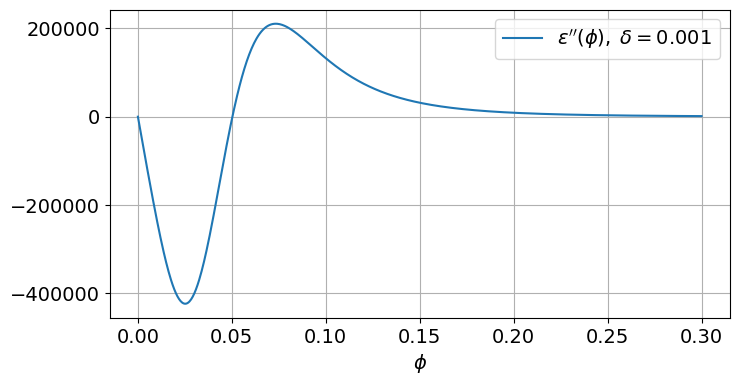
\includegraphics[width=\textwidth]{figures/eps_phi_phi.png}
	\vspace{-0.7cm}
	\caption{Typical behavior of~$\epsilon''(\phi)$ in the vicinity of~$0$.}
	\label{fig:eps_phi_phi}
\end{figure}

To proceed let us estimate extremums of~$\epsilon''(\phi)$ in the neighbourhood of~$0$.
First, find zeros of~$\epsilon'''(\phi)$. We have
\begin{equation}
	\epsilon''' = \epsilon_0 \cfrac{-6 (f')^3 + 6 (f + \delta) f' f'' - (f + \delta)^2 f'''}{(f + \delta)^4},
	\label{eq:epsilon_phi_phi_phi}
\end{equation}
form where:
$$\epsilon'''(\phi) = -6 (f')^3 + 6 (f + \delta) f' f'' - (f + \delta)^2 f''' = 0 \tcomma$$
or, taking~\eqref{eq:epsilon} into account:
$$-3 \cdot 12^2 (1 - \phi)^3 + 36 \left(4 - 3\phi + \cfrac{\delta}{\phi^3} \right)(1 - \phi)(2 - 3\phi) - \left(4 - 3 \phi + \cfrac{\delta}{\phi^3} \right)^2 (1 - 3 \phi) = 0 \tpoint$$

Let~$\delta_n \to +0$ and~$\phi_n \to +0$ such that~$\delta_n / \phi_n^3$ is bounded.
Then:
\begin{gather*}
	-3 \cdot 12^2 \cdot 1^3 + 36 \left(4 + \cfrac{\delta_n}{\phi_n^3} \right) \cdot 1 \cdot 2 - \left(4 + \cfrac{\delta_n}{\phi_n^3} \right)^2 \cdot 1 \to 0 \tcomma \\
	\left(4 + \cfrac{\delta_n}{\phi_n^3} \right)^2 - 72 \left(4 + \cfrac{\delta_n}{\phi_n^3} \right) + 3 \cdot 12^2 \to 0 \tpoint
\end{gather*}
Hence, a sequence~$4 + \delta_n / \phi_n^3$ has not more than two partial limits~$\xi_+$ and~$\xi_-$~---
which are zeros of the equation~$\xi^2 - 72 \xi + 432 = 0$.
To the first zero~$\xi_+ = 36 + 12 \sqrt{6}$ it corresponds
$$\phi_+ = \cfrac{1}{\sqrt[3]{32 + 12 \sqrt{6}}} \sqrt[3]{\delta_n} \approx \cfrac{1}{3.945} \sqrt[3]{\delta_n} \tsemicolon$$
to the second zero~$\xi_- = 36 - 12 \sqrt{6}$ it corresponds
$$\phi_- = \cfrac{1}{\sqrt[3]{32 - 12 \sqrt{6}}} \sqrt[3]{\delta_n} \approx \cfrac{1}{1.376} \sqrt[3]{\delta_n} \tpoint$$

From here it can be seen that for~$\delta \to +0$ the function~$\epsilon'''(\phi)$ has two zeros in the neighbourhood of~$0$:
\begin{equation}
  \phi_{\pm} = \cfrac{1}{\sqrt[3]{32 \pm 12 \sqrt{6}}} \sqrt[3]{\delta} [1 + o(1)] \tpoint
  \label{eq:epsilon_phi_phi_phi_roots}
\end{equation}

We now estimate~$\epsilon''(\phi)$ at~$\phi_{\pm}$  for~$\delta \to +0$. Let~$\phi = (1 / c) \sqrt[3]{\delta}$, $c \in \Real$.
Then:
$$\epsilon'' = \epsilon_0 \cfrac{24 c^5 (8 - c^3)}{(4 + c^3)^3} \delta^{-5 / 3} [1 + o(1)],$$
and:
\begin{equation}
  \epsilon''(\phi_+) \approx -4.378 \epsilon_0 \delta^{-5 / 3}; \quad \epsilon''(\phi_-) \approx 2.216 \epsilon_0 \delta^{-5 / 3} \tpoint
  \label{est:epsilon_phi_phi_bounds}
\end{equation}
The derived estimates are shown as black dashed lines on Fig.~\ref{fig:eps_phi_phi_multiplied}.

\begin{figure}[!t]
	\centering
	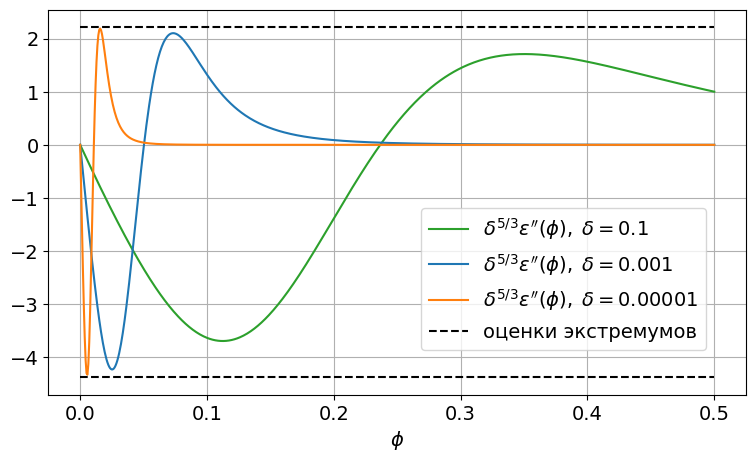
\includegraphics[width=\textwidth]{figures/eps_phi_phi_multiplied.png}
	\caption{Qualitative behavior of~$\delta^{5 / 3} \epsilon''(\phi)$ for small values of~$\delta$.}
	\label{fig:eps_phi_phi_multiplied}
\end{figure}

Now, to derive new stability estimate we consider equation~\eqref{eq:spectral} at~$\phi = \phi_+$.
Note that~$\epsilon''(\phi_+) \approx -4.4 \epsilon_0 \delta^{-5 / 3}$.
The term inside braces in~\eqref{eq:spectral} is negative since
$\delta$ is small and~$\epsilon''(\phi_+)$ is negative and large in its absolute value.
Therefore~$f''(\phi_+) > 0$ can be estimated as~$0$~--- such estimate makes inequality stronger.
Then from inequality~\eqref{eq:spectral} it follows that 
$$\lambda(\theta) = 1 + m \tau \left( -\cfrac{2.2 K_\Phi^2 \epsilon_0}{\delta^{5 / 3}} - \cfrac{2 \Gamma}{h^2} \sin^2 \cfrac{\theta}{2} \right) \tpoint$$
Condition~$|\lambda(\theta)| \leqslant 1$ is satisfied for an arbitrary~$\theta$, if and only if
\begin{equation}
  \tau \leqslant \cfrac{1}{m} \left( \cfrac{1.1 K_\Phi^2 \epsilon_0}{\delta^{5 / 3}} + \cfrac{\Gamma}{h^2} \right)^{-1} \tpoint
  \label{cond:spectral_better_theoretical}
\end{equation}

Numerical experiments described in the next sections indicates that
more strong version of the estimate~\eqref{cond:spectral_better_theoretical} is also valid
(note the doubled denominator):
%
\begin{equation}
  \tau \leqslant \cfrac{1}{2m} \left( \cfrac{K_\Phi^2 \epsilon_0}{\delta^{5 / 3}} + \cfrac{\Gamma}{h^2} \right)^{-1} \tpoint
  \label{cond:spectral_better}
\end{equation}

Finally, more simple estimate not weaker then~\eqref{cond:spectral_better} is:
\begin{equation}
  \tau \leqslant \cfrac{1}{4m} \min \left(\cfrac{\delta^{5 / 3}}{K_\Phi^2 \epsilon_0}, \; \cfrac{h^2}{\Gamma} \right) \tpoint
  \label{cond:spectral_better_simpler}
\end{equation}

Note that the derived stability estimate~\eqref{cond:spectral_better}
for finite-difference scheme~\eqref{sch:transition},\eqref{sch:borders}
includes all the parameters of the equation~\eqref{eq:one_dim}, except~$l$.
Notably, this is the only parameter of the model which has somehow artificial nature and can not be
related directly to the underlying physics.

\endinput
% EOF

\clearpage
\printbibliography[
	heading=bibintoc
]

\clearpage
\tableofcontents

\end{document}

%%%%%%%%%%%%%%%%%%%%%%%%%%%%%%%%%%%%%%%%%%%%%%%%%%%%%%%%%%%%%%%%%%%%%%%%%%%%%%%%